\section{Phase 4: LLM Response Evaluation}
\label{sec:phase4-llm-evaluation}

In this phase, participants were asked to evaluate the responses generated by the language model based on the procedure outlined in Section~\ref{sec:phase4-llm-responses}. The responses were assessed using a Likert scale across four criteria: \textit{Relevance}, \textit{Emotional Alignment}, \textit{Empathy}, and \textit{Satisfaction}. Each participant rated responses to both a standard (controlled) query and an emotionally-enhanced query.

This evaluation allowed us to compare how the emotional enhancement influenced user perception of the generated responses. The comparison of average ratings between the two types of queries across all four evaluation dimensions is illustrated in Figure~\ref{fig:llm_eval_comparison}.

\begin{figure}[h]
    \centering
    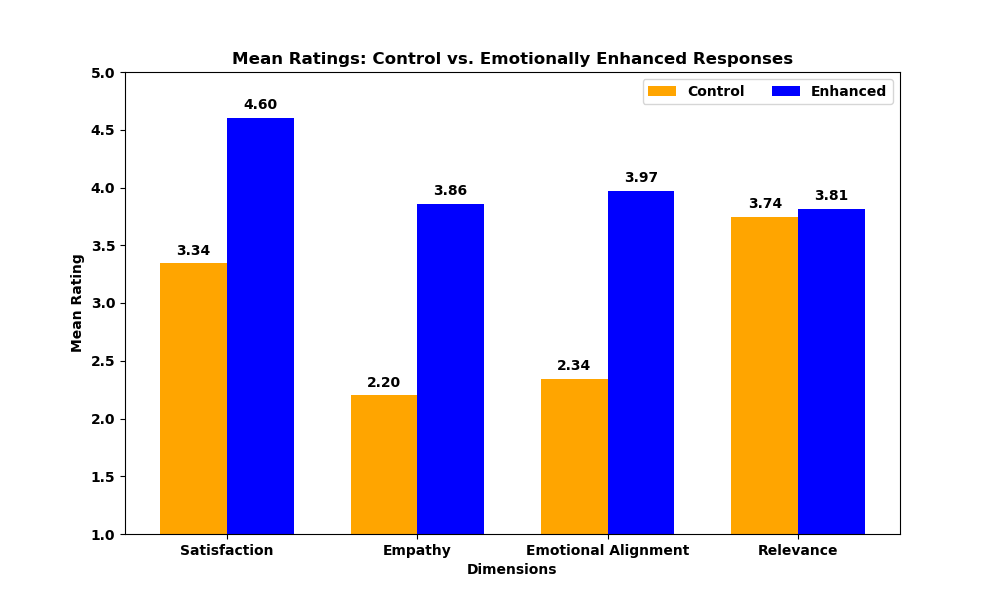
\includegraphics[width=1\textwidth]{img/chapter_04/llm/mean_ratings_comparison.png}
    \caption{Comparison of average ratings for LLM responses}
    \label{fig:llm_eval_comparison}
\end{figure}

\subsection*{Overall Analysis Results}

\begin{table}[H]
    \centering
    \begin{tabular}{|l|c|c|c|c|}
    \hline
    \textbf{Dimension} & \textbf{\makecell{Mean\\Control}} & \textbf{\makecell{Mean\\Enhanced}} & \textbf{\makecell{Mean\\Difference}} & \textbf{\makecell{Improvement\\(\%)}} \\
    \hline
    Satisfaction        & 3.343 & 4.600 & 1.257 & 37.6 \\
    Empathy             & 2.200 & 3.857 & 1.657 & 75.3 \\
    Emotional Alignment & 2.343 & 3.971 & 1.629 & 69.5 \\
    Relevance           & 3.743 & 3.814 & 0.071 & 1.9  \\
    \hline
    \end{tabular}
    \caption{Comparison of participant evaluations for control vs emotionally enhanced responses}
    \label{tab:llm_overall_analysis}
\end{table}


As seen in Table~\ref{tab:llm_overall_analysis}, there is a clear overall increase in user satisfaction, indicating a robust and consistent enhancement in user experience when emotional tailoring is applied. This suggests that emotionally enhanced responses are more engaging and fulfilling for users across various types of queries.

The most significant improvements are observed in \textit{Empathy} (75.3\%) and \textit{Emotional Alignment} (69.5\%), followed by \textit{Satisfaction} (37.6\%). These dimensions, being closely linked to subjective and emotional user experiences, benefit substantially from emotional enhancement. 

On the other hand, the impact on \textit{Relevance} is limited. With only a 1.9\% improvement and a low proportion of participants reporting a positive change as relevance is more dependent on content correctness, which was already adequately addressed by the control responses.
